\begin{figure}[t]
  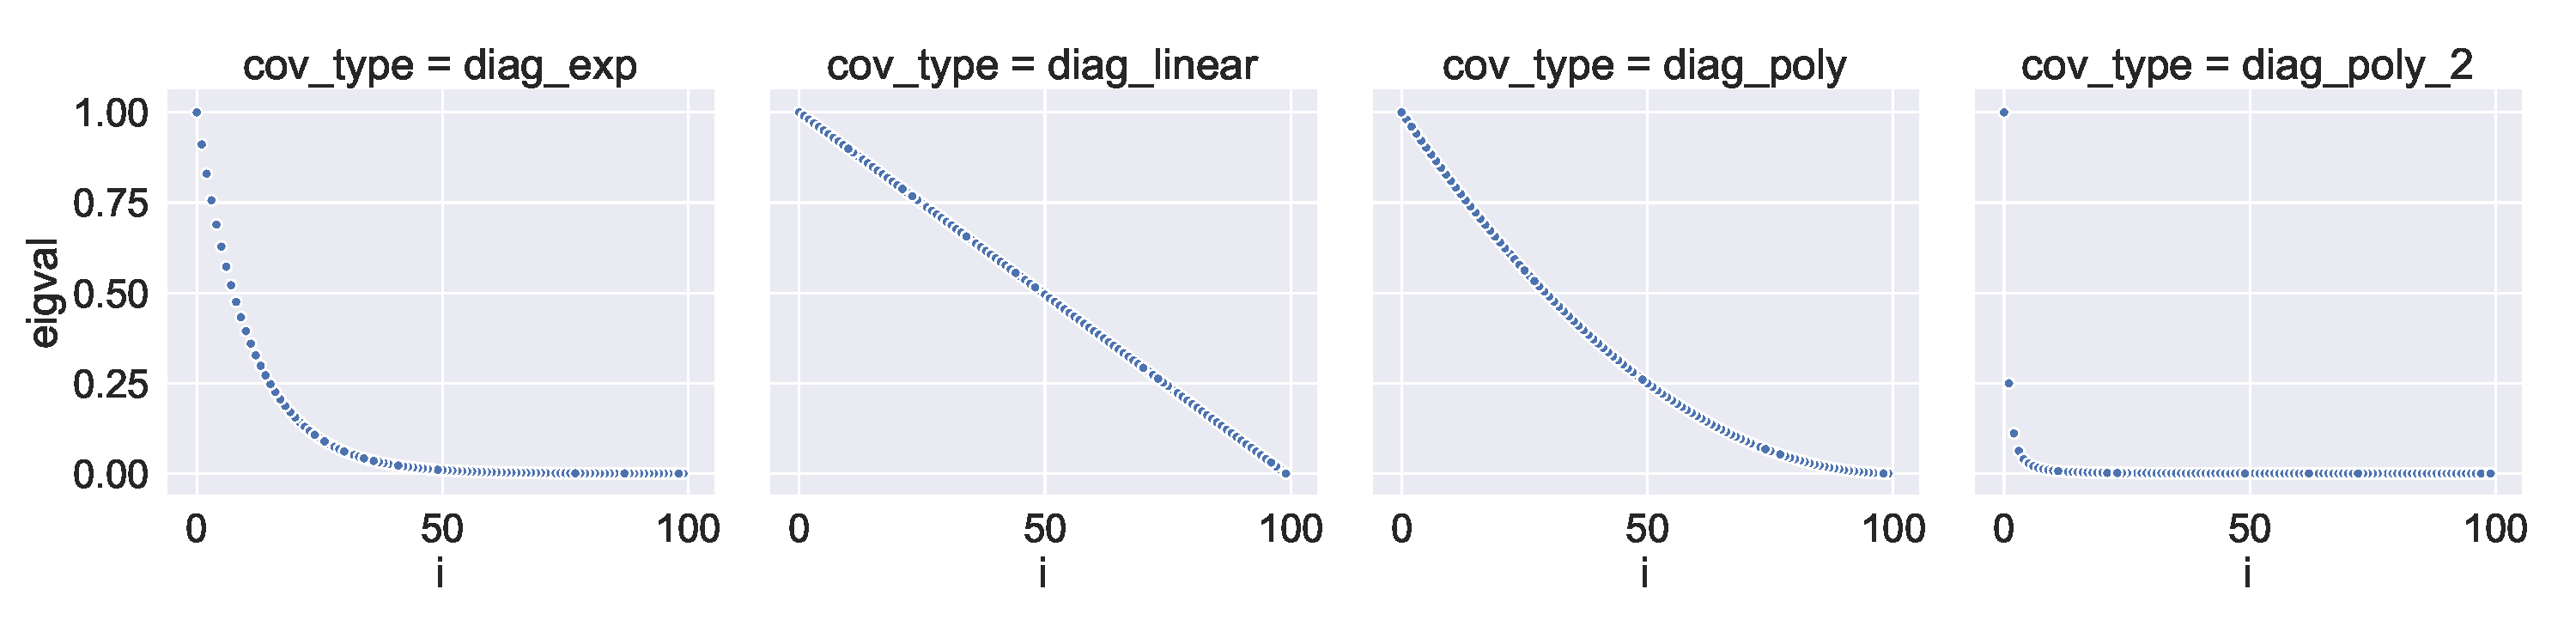
\includegraphics[width=\textwidth]{design/continuous_figures/decays.pdf}
  \vspace{-1cm}
  \caption{Scree-plots of $\Sigmab$ for the eigenvalue decays examined
    in our empirical valuations.
    % Here $d=100$ for visualization, whereas
    % our experiments increase $d$ while preserving the ratio $n/d$ and
    % the decay profile,
    % with $\lambda_{\text{max}}(\Sigmab) = 1$ to
    % $\lambda_{\text{min}}(\Sigmab) = 10^{-4}$.
  }
  \label{fig:eig-decays}
\end{figure}


\section{Empirical evaluation of asymptotic consistency}
\label{sec:asymp-conj-details}

% While Theorem~\ref{t:asymptotic} is a result on asymptotic consistency of the
% MSE, the proof (Appendix~\ref{sec:proof-of-t-asymptotic}) follows the standard
% decomposition of MSE in Equation~\ref{eq:mse-derivation} in the process
% establish consistency on the bias and variance terms independently.

% Recall that $\lambda_n=\frac {d-n}{\tr((\Sigmab+\lambda_n\I)^{-1})}$,
% so our surrogate MSE is recovered as
% $\sigma^2\Vc(\Sigmab,n)+\w^{*\top}\Bc(\Sigmab,n)\w^*$.
% % The expressions $\Vc(\Sigmab,n)$ and $\Bc(\Sigmab,n)$ and recover
% % surrogate MSE from Theorem \ref{t:mse} since $\lambda_n=\frac{\tr((\Sigmab+\lambda_n)^{-1})}{d-n}$.
% Lemmas \ref{c:wishart} and \ref{c:projection} provide new insights into classical matrix-variate
% distributions with extensive literature dedicated to them \citep[see,
% e.g.,][]{chikuse1990matrix,cook2011}.
%
%
%

%\section{Empirical evaluation of asymptotic consistency}

% Theorem \ref{t:asymptotic} shows that the surrogate MSE expressions
% derived in Theorem \ref{t:mse} are asymptotically consistent with the
% true MSE for the i.i.d.~design under a class of sub-gaussian data
% distributions.
In this section, we empirically quantify the convergence rates for
the asymptotic result of Theorem~\ref{t:asymptotic}.
% when $\mu$ is a centered multivariate% Gaussian $\Nc(\zero,\Sigmab).$
We focus on the under-determined regime (i.e.,
$n<d$) and separate the evaluation into the bias and
variance terms, following the MSE decomposition given
in \eqref{eq:mse-derivation}. Consider  $\X = \Z\Sigmab^{1/2} $, where the entries of $\Z$ are
i.i.d. standard Gaussian, and define:\vspace{-1mm}
\begin{enumerate}
  \item Variance discrepancy:\quad
        $\big|\frac{\E[\tr((\X^\top\X)^\dagger)]}{\Vc(\Sigmab,n)}-1\big|$ where
        $\Vc(\Sigmab,n)=\frac{1-\alpha_n}{\lambda_n}$.
  \item Bias discrepancy:\quad
        $\sup_{\w\in\R^d\backslash\{\zero\}}\big|\frac{\w^\top\E[\I-\X^\dagger\X]\w}
          {\w^\top\Bc(\Sigmab,n)\w} - 1\big|$
        where $\Bc(\Sigmab,n) = \lambda_n(\Sigmab+\lambda_n\I)^{-1}$.
\end{enumerate}\vspace{-1mm}
Recall that $\lambda_n=\frac {d-n}{\tr((\Sigmab+\lambda_n\I)^{-1})}$,
so our surrogate MSE can be written as
$\Mc=\sigma^2\Vc(\Sigmab,n)+\w^{*\top}\Bc(\Sigmab,n)\w^*$, and when both
discrepancies are bounded by $\epsilon$, then $(1-2\epsilon)\Mc\leq\MSE{\X^\dagger\y}\leq (1+2\epsilon)\Mc$.
In our experiments, we consider four standard eigenvalue decay profiles
for $\Sigmab$, including polynomial and exponential decay (see
\Cref{fig:eig-decays} and \Cref{sec:eig-decay-details}).
\begin{figure} %[ht]
  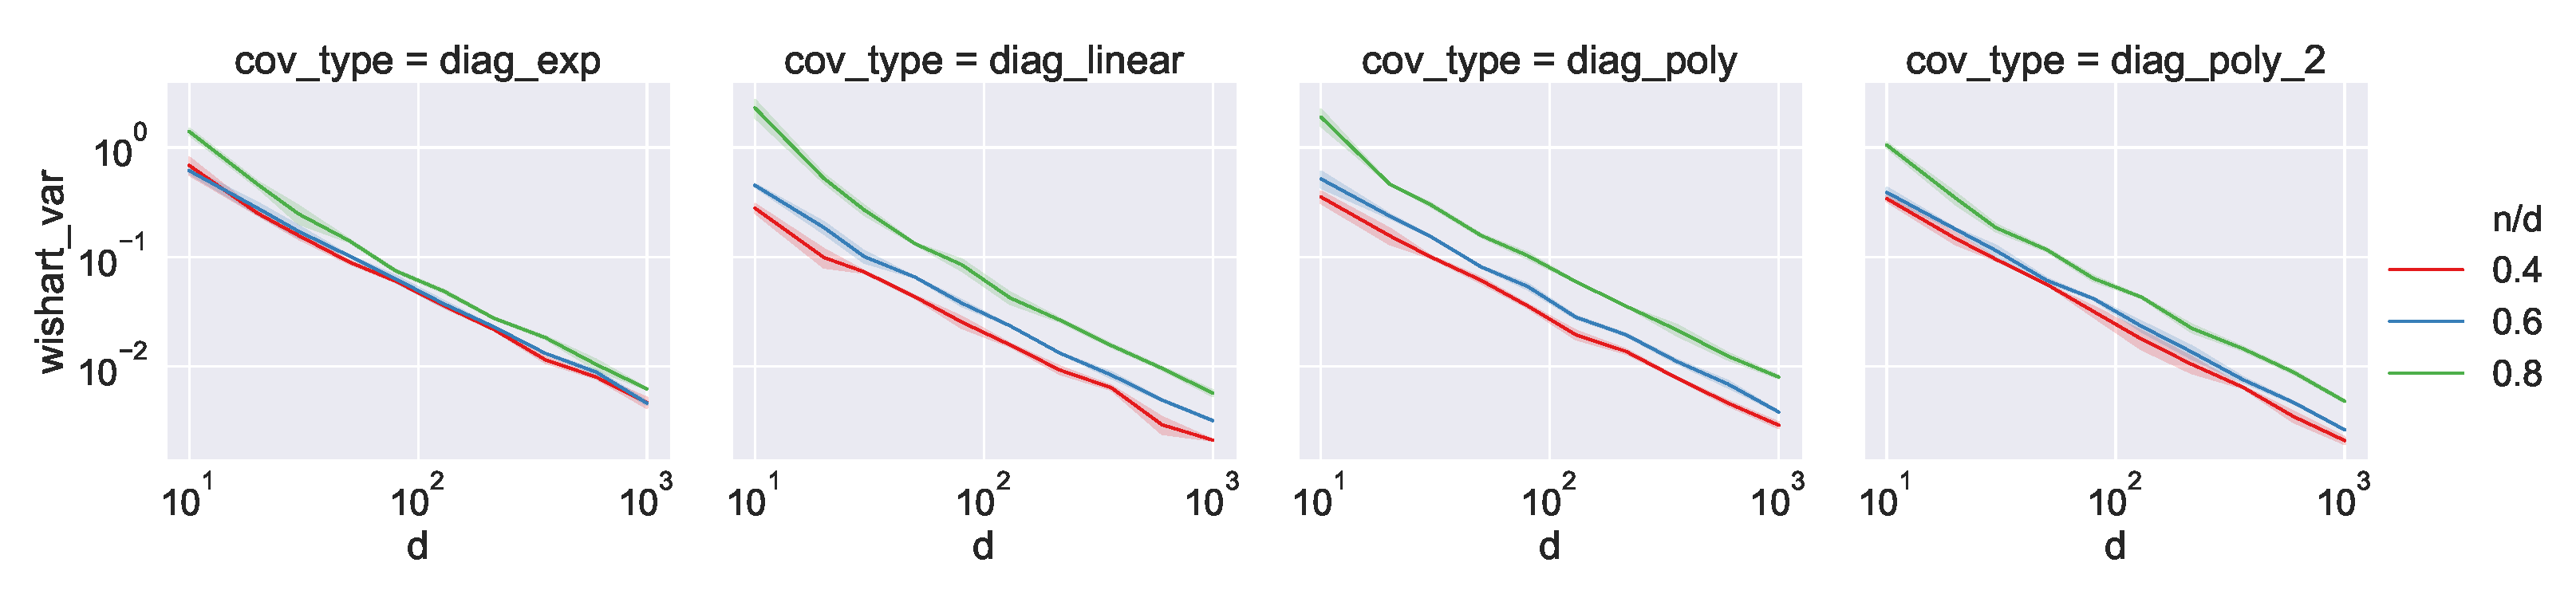
\includegraphics[width=\textwidth]{design/continuous_figures/wishart_var.pdf}
  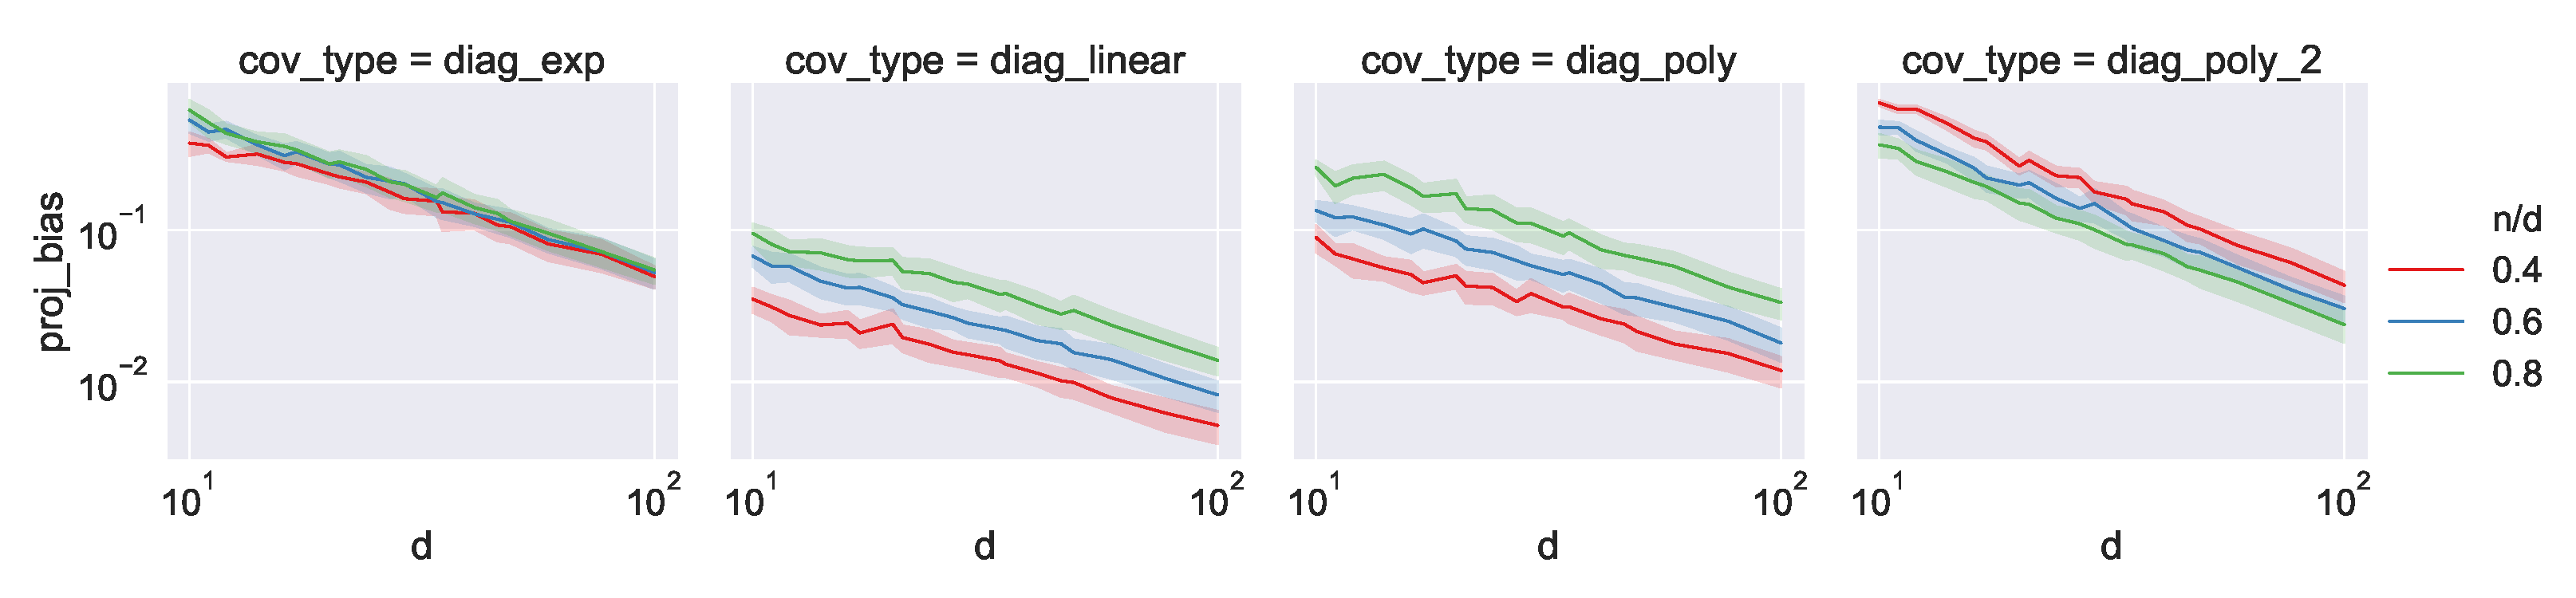
\includegraphics[width=\textwidth]{design/continuous_figures/proj_bias.pdf}
  \vspace{-.8cm}
  \caption{
    Empirical verification of the asymptotic consistency of surrogate MSE.
    We show the discrepancies for the variance (top) and bias
    (bottom),  with bootstrapped $95\%$ confidence intervals, as $d$
    increases and $n/d$ is fixed. We observe
    $O(1/d)$ decay (linear with slope $-1$ on a log-log plot).
  }
  \label{f:conj-wishart}
\end{figure}

Figure~\ref{f:conj-wishart} (top) plots the variance discrepancy (with
$\E[\tr((\X^\top\X)^\dagger)]$ estimated via Monte Carlo
sampling and bootstrapped confidence intervals) as $d$ increases from $10$ to
$1000$, across a range of aspect ratios $n/d$. In all cases, we observe that
the discrepancy decays to zero at a rate of $O(1/d)$.
Figure~\ref{f:conj-wishart} (bottom) plots the bias discrepancy, with the same
rate of decay observed throughout.  Note that the range of $d$ is smaller than
in Figure \ref{f:conj-wishart} (top) because the large number of Monte Carlo
samples (up to two million) required for this experiment made the computations
much more expensive (more details in \Cref{a:empirical}). Based on the
above empirical results, we conclude with a conjecture.
\begin{conjecture}
  \label{c:1-over-d-rate}
  When $\mu$ is a centered multivariate Gaussian and its covariance
  has a constant condition
  number, then, for $n/d$ fixed, the surrogate MSE satisfies:
  $\big|\frac{\textnormal{MSE}[\X^\dagger\y]}{\Mc}-1\big|= O(1/d)$.
\end{conjecture}

% The results of empirically validating \Cref{c:wishart} are illustrated in
% Figure~\ref{f:conj-wishart} (top), where we performed Monte Carlo estimation of
% $\E\big[\tr((\X^\top\X)^\dagger)\big]$ and plot
% $\big|\E[\tr((\X^\top\X)^\dagger)]\,\Vc(\Sigmab,n)^{-1} -1\big|$ as $d$ increases from
% $10$ to $1000$, across a range of aspect ratios $n/d$ and eigenvalue decay
% profiles for $\Sigmab$.
% We observe that on log-log axes all of the plots are
% decreasing with a linear $-1$ slope, consistent with the $O(1/d)$ rate
% predicted by \Cref{c:wishart}. \Cref{c:projection} is handled similarly, by
% sampling $\X\sim\mu^n$ where $\mu=\Nc(\zero,\Sigmab )$ to obtain a Monte Carlo
% estimate of $\E[\I-\X^\dagger\X]$.

% Figure~\ref{f:conj-wishart} (bottom) shows how \eqref{eq:projection} decays as
% we hold the aspect ratio $n/d$ fixed and increase $d$ between $10$ and $100$
% across the listed eigenvalue decay profiles and aspect ratios. Again, we
% observe on log-log axes a linear decay with slope $-1$ consistent with the
% $O(1/d)$ rate posed by \Cref{c:projection}. Note that the range of $d$ is
% smaller than in Figure \ref{f:conj-wishart} (top) because the large number of
% Monte Carlo samples (up to two million) required for this experiment made the
% computations much more expensive.


\subsection{Additional details for empirical evaluation}
\label{a:empirical}

Our empirical investigation of the rate of asymptotic convergence in \Cref{t:asymptotic} (and, more
specifically, the variance and bias discrepancies defined in
Section~\ref{sec:asymp-conj-details}), in the context of
Gaussian random matrices, is related to open problems which have been
extensively studied in the literature. Note that when
$\X=\Z\Sigmab^{1/2}$ were $\Z$ has i.i.d.~Gaussian entries (as in
Section \ref{sec:asymp-conj-details}), then $\W=\X^\top\X$ is known as the
pseudo-Wishart distribution (also called the singular Wishart),
denoted as $\W \sim \Pc\Wc(\Sigmab, n)$, and the variance
term from the MSE can be written as $\sigma^2\E[\tr(\W^\dagger)]$.
\cite{srivastava2003} first derived the probability density function of the
pseudo-Wishart distribution, and
\cite{cook2011} computed the first and second moments of generalized
inverses. However, for the Moore-Penrose inverse and arbitrary
covariance $\Sigmab$, \cite{cook2011} claims that the quantities required to
express the mean ``do not have tractable closed-form representation.''
The bias term, $\w^{*\top}\E[\I-\X^\dagger\X]\w^*$, has connections to
directional statistics.  Using the SVD,
we have the equivalent representation $\X^\dagger \X = \V \V^\top$ where $\V$
is an element of the Stiefel manifold $V_{n,d}$ (i.e., orthonormal $n$-frames
in $\R^d$).  The distribution of $\V$ is known as the matrix angular central
Gaussian (MACG) distribution \citep{chikuse1990matrix}. While prior work has
considered high dimensional limit theorems \citep{CHIKUSE1991145} as well as
density estimation and hypothesis testing \citep{CHIKUSE1998188} on $V_{n,d}$,
they only analyzed the invariant measure (which corresponds in our setting to
$\Sigmab = \I$), and to our knowledge a closed form expression of
$\E[\V\V^\top]$ where $\V$ is distributed according to MACG with arbitrary
$\Sigmab$ remains an open question.

For analyzing the rate of decay of variance and bias discrepancies (as
defined in Section \ref{sec:asymp-conj-details}), it suffices to only consider diagonal
covariance matrices $\Sigmab$.  This is because if $\Sigmab = \Q \D \Q^\top$ is
its eigendecomposition and $\X\sim\Nc_{n,d}(\zero, \I_n \otimes \Q\D\Q^\top)$,
then we have for $\W \sim \Pc\Wc(\Sigmab, n)$ that $\W \overset{d}{=} \X^\top
  \X$ and hence, defining $\Xt\sim\Nc_{n,d}(\zero,\I_n \otimes \D)$, by linearity
and unitary invariance of trace,
\begin{align*}
  \E[\tr(\W^\dagger)]
   & = \tr\big( \E[(\X^\top\X)^\dagger] \big)
  = \tr\Big( \Q\E\big[(\Xt^\top\Xt)^\dagger\big]\Q^\top \Big)
  = \tr\Big( \E\big[(\Xt^\top\Xt)^\dagger\big] \Big)
  = \E\left[\tr \big((\Xt^\top\Xt)^\dagger\big) \right].
\end{align*}
Similarly, we have that $\E[\X^\dagger\X]=\Q\E\big[\Xt^\dagger\Xt\big]\Q^\top$,
and a simple calculation shows that the bias discrepancy is
also independent of the choice of matrix $\Q$.

In our experiments, we increase $d$ while keeping the aspect ratio $n/d$
fixed and examining the rate of decay of the discrepancies.
We estimate $\E\big[\tr(\W^\dagger)\big]$ (for the variance) and
$\E[\I-\X^\dagger\X]$ (for the bias) through Monte Carlo sampling.
Confidence intervals are constructed using ordinary bootstrapping for
the variance. We rewrite the supremum over $\w$ in bias discrepancy as
a spectral norm:
\[\big\|\Bc(\Sigmab,n)^{-\frac12}\E[\I-\X^\dagger\X]\Bc(\Sigmab,n)^{-\frac12} -
  \I\big\|,\]
and apply existing methods for constructing bootstrapped operator
norm confidence intervals described in \cite{lopes2019bootstrapping}.  To
ensure that estimation noise is sufficiently small, we continually increase the
number of Monte Carlo samples until the bootstrap confidence intervals are
within $\pm 12.5\%$ of the measured discrepancies.  We found that while
variance discrepancy required a relatively small number of trials (up
to one thousand), estimation noise was much larger for the bias
discrepancy, and it necessitated over two million trials to obtain
good estimates near $d=100$.

\subsection{Eigenvalue decay profiles}
\label{sec:eig-decay-details}

Letting $\lambda_i(\Sigmab)$ be the $i$th largest eigenvalue of
$\Sigmab$, we consider the
following eigenvalue profiles (visualized in Figure~\ref{fig:eig-decays}):
\begin{itemize}
  \item \texttt{diag\_linear}: linear decay, $\lambda_i(\Sigmab)= b-a i$;
  \item \texttt{diag\_exp}: exponential decay, $\lambda_i(\Sigmab) = b\,10^{- a i} $;
  \item \texttt{diag\_poly}: fixed-degree polynomial decay, $\lambda_i(\Sigmab) = (b-a i)^2$;
  \item \texttt{diag\_poly\_2}: variable-degree polynomial decay, $\lambda_i(\Sigmab) = b i^{-a}$.
\end{itemize}
The constants $a$ and $b$ are chosen to ensure $\lambda_{\text{max}}(\Sigmab) = 1$ and
$\lambda_{\text{min}}(\Sigmab) = 10^{-4}$ (i.e., the condition number
$\kappa(\Sigmab) = 10^{4}$ remains constant).
